% !Mode:: "TeX:UTF-8" 



\BiSection{2.24}{Figures}

\fancyhead[R]{本题2.24由QC.Z完成}



解:

\scalebox{3}{(a)}

重画电路于图1

		\begin{figure}[H] %H为当前位置,!htb为忽略美学标准,htbp为浮动图形
	\begin{minipage}{\linewidth}
		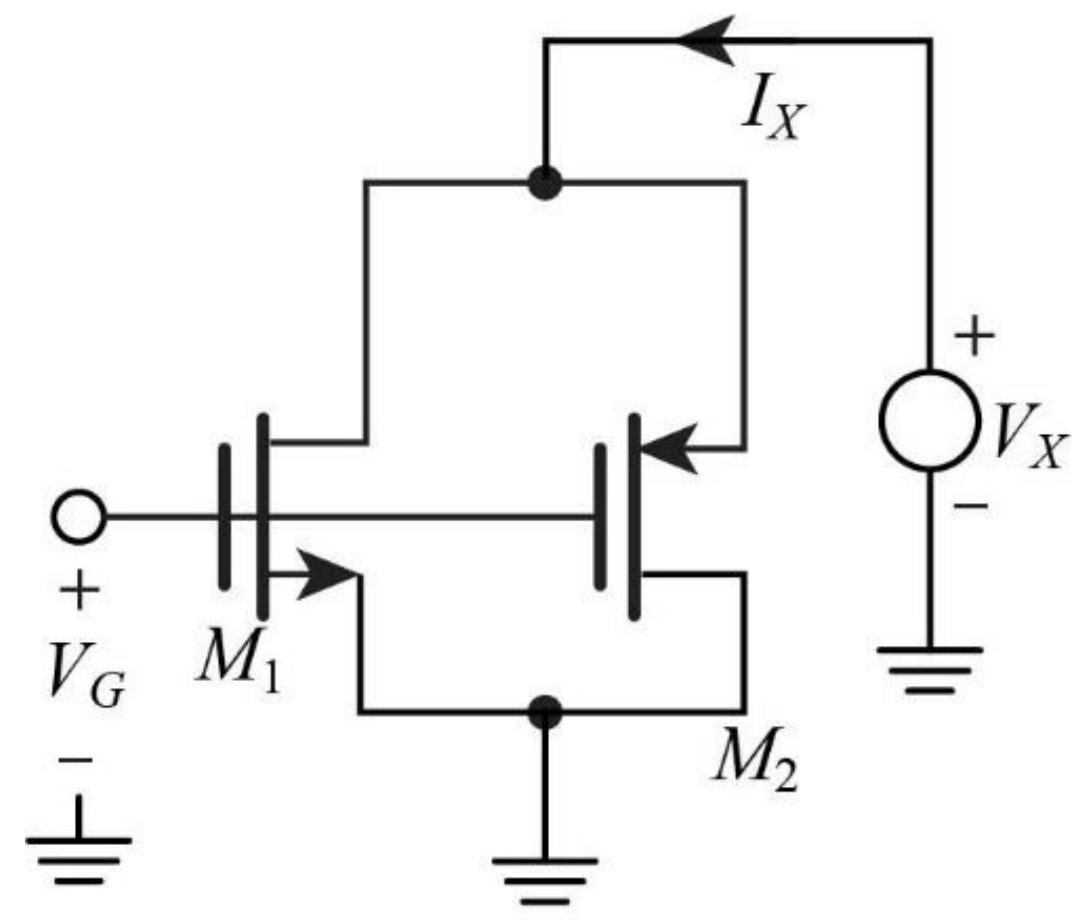
\includegraphics[width=1\linewidth]{2.24-1}
	\end{minipage}
	\caption*{图1} %最终文档中希望显示的图片标题
\end{figure}

\scalebox{2}{(1)}

当$V_G<V_{THN}$时,$M_1$关,$I_{D1}\cong 0A$

对$0<V_X<V_G+|V_{THP}|$:$M_2$关,$I_X\cong 0A$,因为$g_m=\frac{\partial I_X}{\partial V_G}$,所以$g_m=0$

对$V_G+|V_{THP}|<V_X$:$I_X=\frac{1}{2}\mu_pC_{ox}(\frac{W}{L})_p(V_{X}-V_G-|V_{THP}|)^2$

		\begin{figure}[H] %H为当前位置,!htb为忽略美学标准,htbp为浮动图形
	\begin{minipage}{\linewidth}
		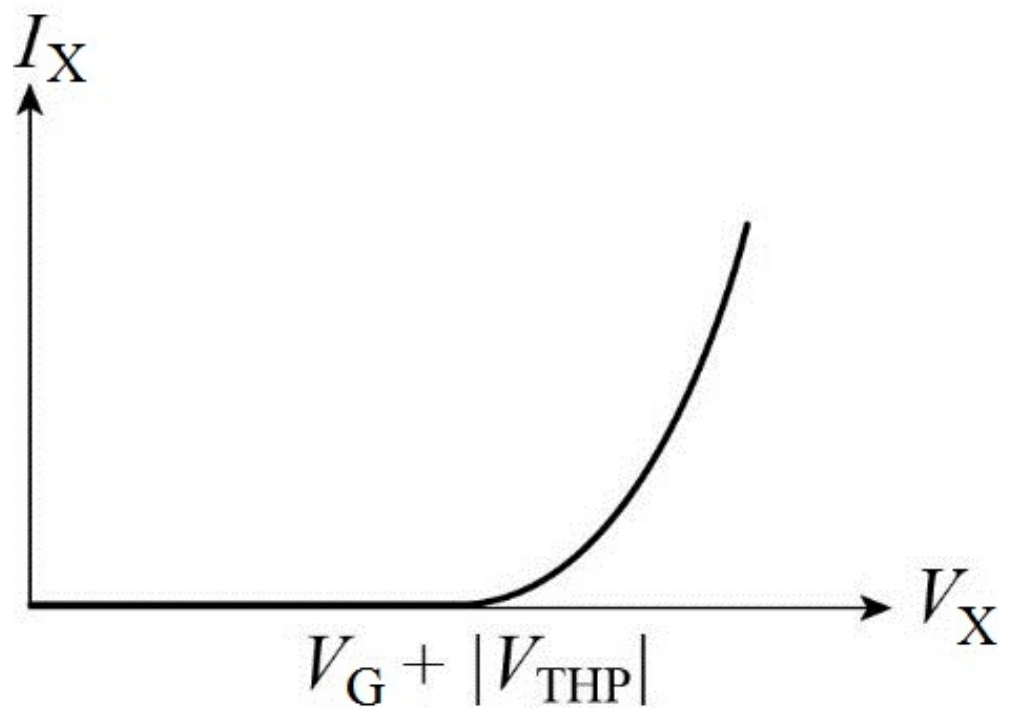
\includegraphics[width=1\linewidth]{2.24-2}
	\end{minipage}
	\caption*{图2} %最终文档中希望显示的图片标题
\end{figure}

		\begin{figure}[H] %H为当前位置,!htb为忽略美学标准,htbp为浮动图形
	\begin{minipage}{\linewidth}
		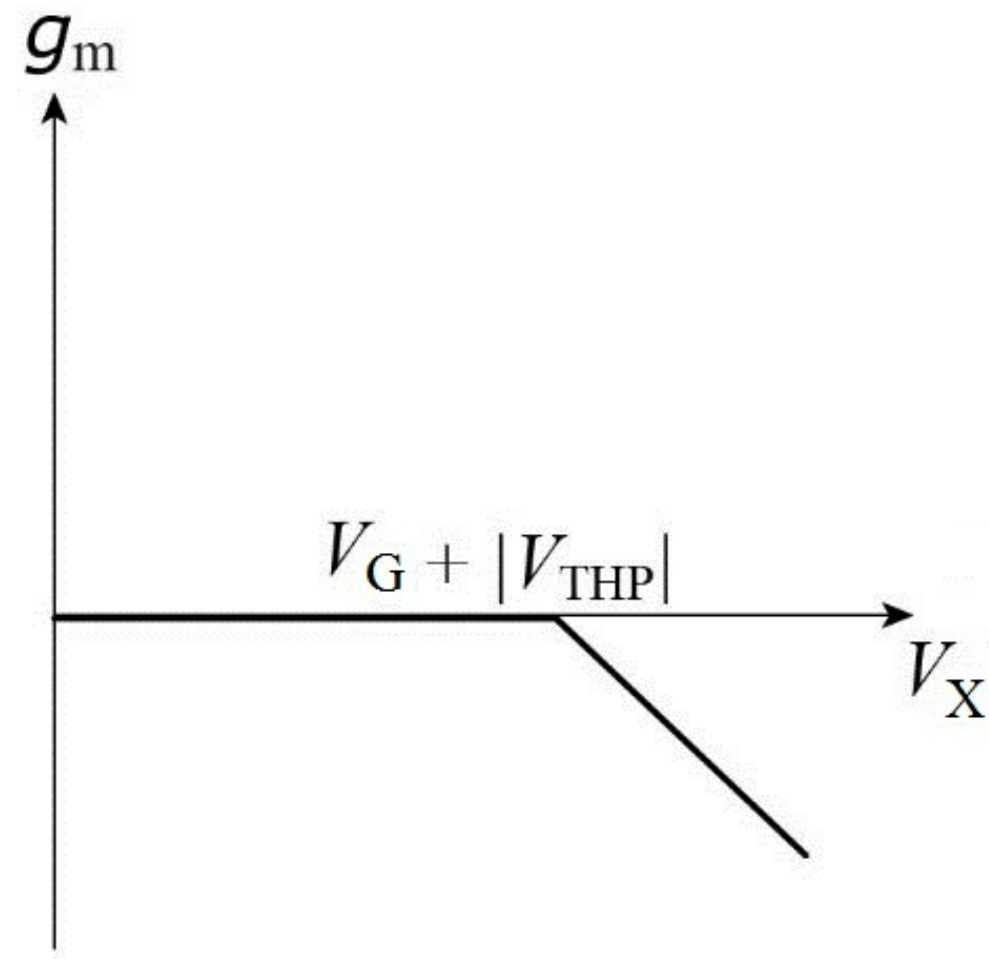
\includegraphics[width=1\linewidth]{2.24-3}
	\end{minipage}
	\caption*{图3} %最终文档中希望显示的图片标题
\end{figure}



\scalebox{2}{(2)}

当$V_G>V_{THN}$时,$M_2$关

对$0<V_X<V_G-|V_{THN}|$:$M_1$在线性区,$M_2$关。

$I_X=\frac{1}{2}\mu_nC_{ox}(\frac{W}{L})_n[2(V_G-V_{THN})V_X-V^2_X]$

\begin{figure}[H] %H为当前位置,!htb为忽略美学标准,htbp为浮动图形
	\begin{minipage}{\linewidth}
		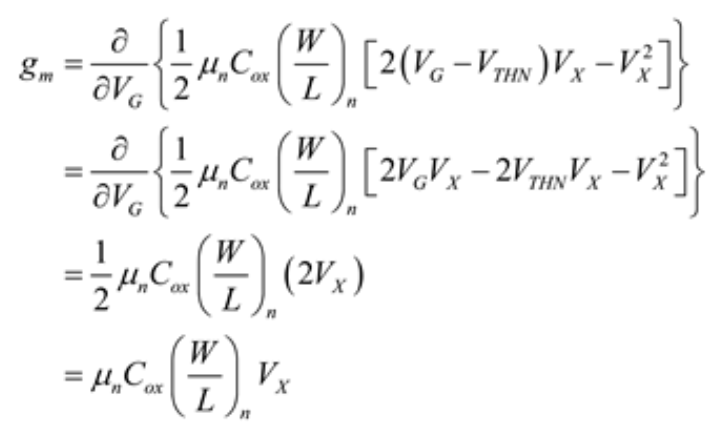
\includegraphics[width=1\linewidth]{2.24-4}
	\end{minipage}
\end{figure}

对$V_G-|V_{THN}|<V_X<V_G+|V_{THP}|$:$M_1$在饱和区,$M_2$关。

$I_X=\frac{1}{2}\mu_nC_{ox}(\frac{W}{L})_n(V_G-V_{THN})^2$

\begin{figure}[H] %H为当前位置,!htb为忽略美学标准,htbp为浮动图形
	\begin{minipage}{\linewidth}
		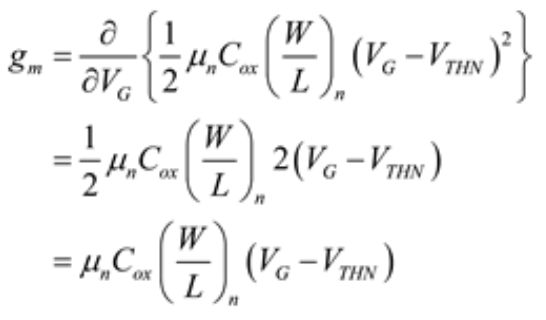
\includegraphics{2.24-5}
	\end{minipage}
\end{figure}

对$V_G+|V_{THP}|<V_X$:$M_1$和$M_2$在饱和区。

$I_X=\frac{1}{2}\mu_nC_{ox}(\frac{W}{L})_n(V_G-V_{THN})^2+\frac{1}{2}\mu_pC_{ox}(\frac{W}{L})_p(V_{X}-V_G-|V_{THP}|)^2$

\begin{figure}[H] %H为当前位置,!htb为忽略美学标准,htbp为浮动图形
	\begin{minipage}{\linewidth}
		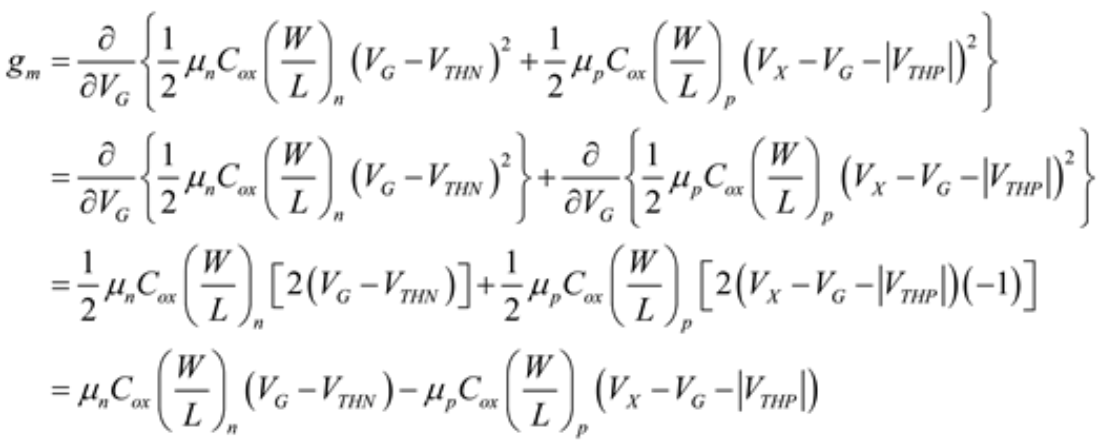
\includegraphics[width=1\linewidth]{2.24-6}
	\end{minipage}
\end{figure}

		\begin{figure}[H] %H为当前位置,!htb为忽略美学标准,htbp为浮动图形
	\begin{minipage}{\linewidth}
		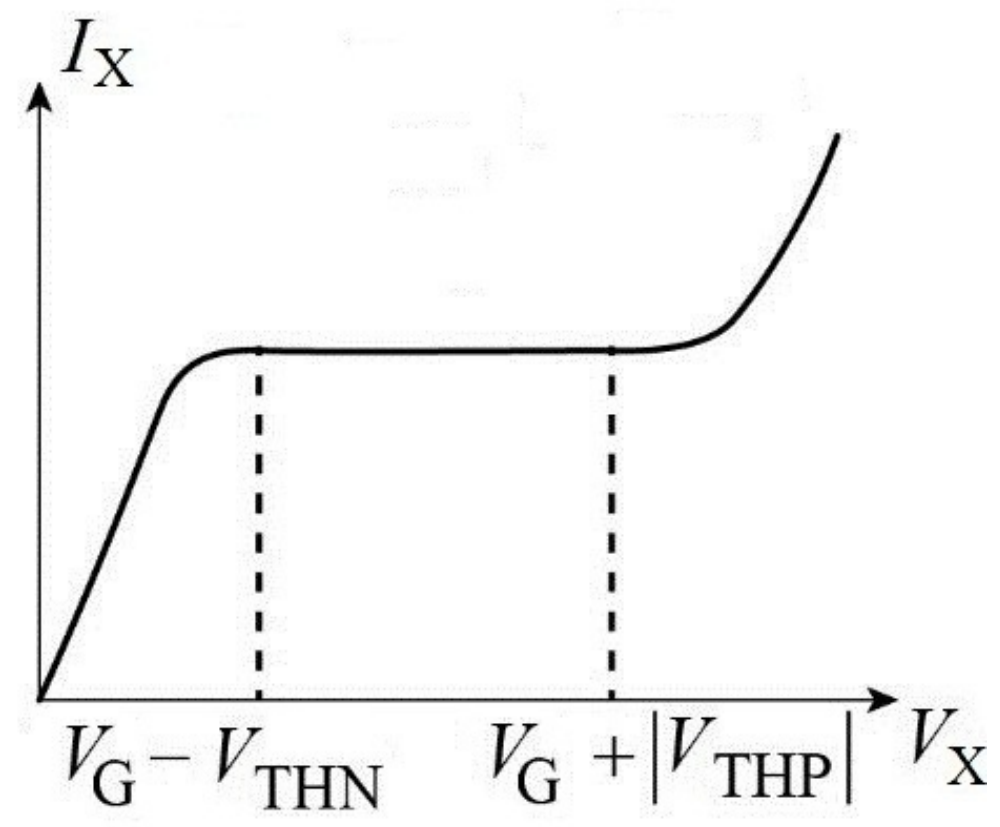
\includegraphics[width=1\linewidth]{2.24-7}
	\end{minipage}
	\caption*{图4} %最终文档中希望显示的图片标题
\end{figure}

		\begin{figure}[H] %H为当前位置,!htb为忽略美学标准,htbp为浮动图形
	\begin{minipage}{\linewidth}
		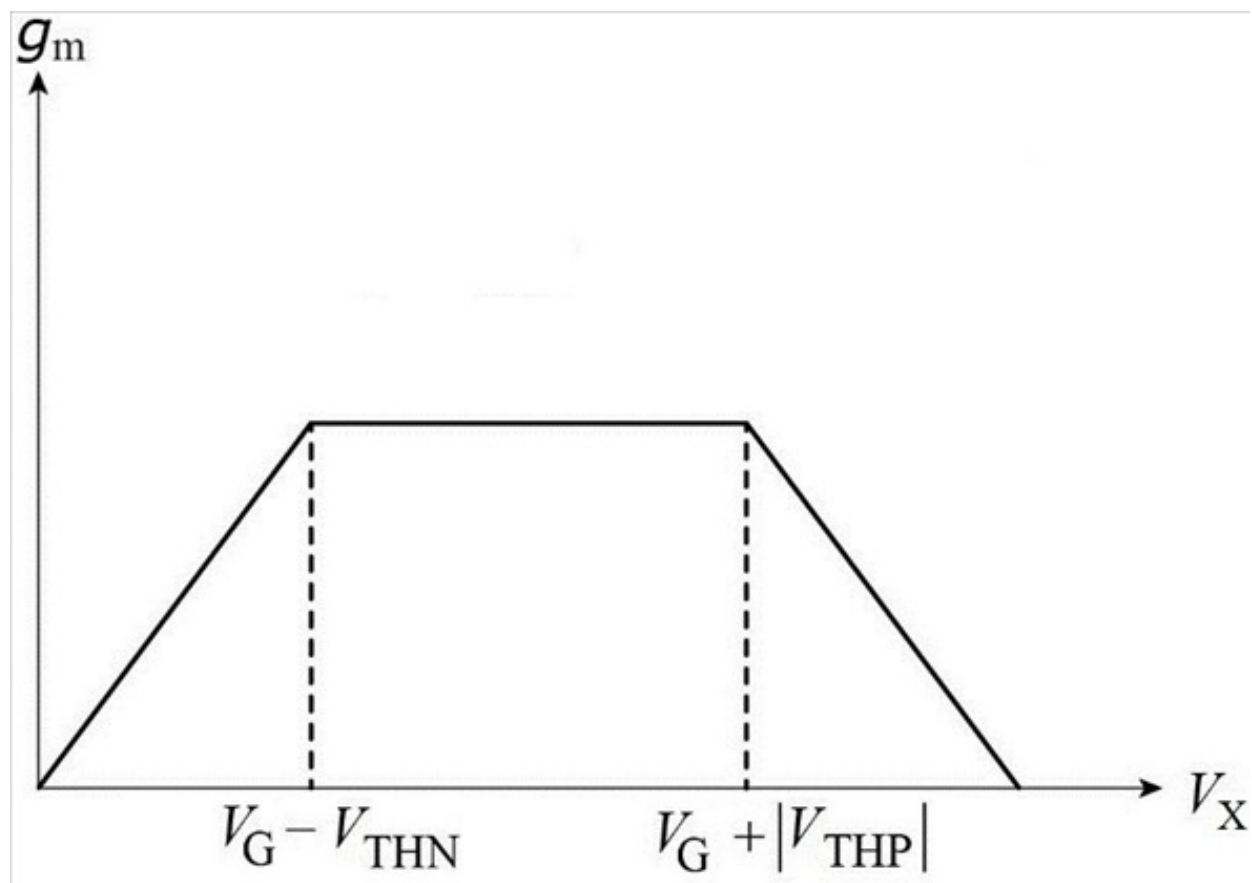
\includegraphics[width=1\linewidth]{2.24-8}
	\end{minipage}
	\caption*{图5} %最终文档中希望显示的图片标题
\end{figure}

\scalebox{3}{(b)}

重画电路于图6

\begin{figure}[H] %H为当前位置,!htb为忽略美学标准,htbp为浮动图形
	\begin{minipage}{\linewidth}
		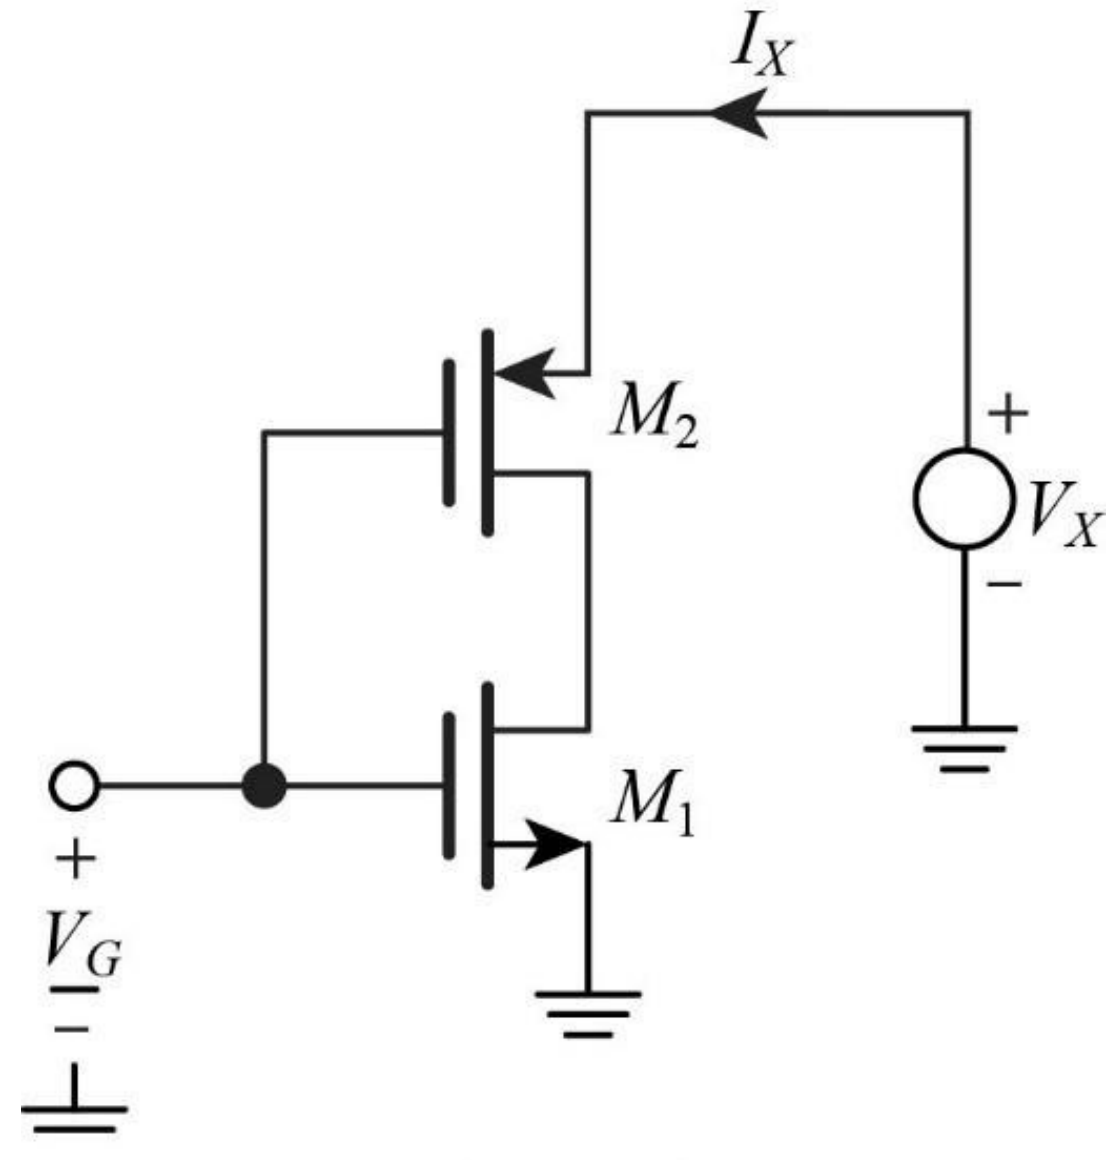
\includegraphics[width=1\linewidth]{2.24-9}
	\end{minipage}
	\caption*{图6} %最终文档中希望显示的图片标题
\end{figure}

\scalebox{2}{(1)}

当$V_G<V_{THN}$时,$M_1$关,$I_X\cong 0A$,因为$g_m=\frac{\partial I_X}{\partial V_G}$,所以$g_m=0$

\scalebox{2}{(2)}

当$V_G>V_{THN}$时,$M_2$关

对$0<V_X<V_G+|V_{THP}|$:$M_2$关,$I_X\cong 0A$,因为$g_m=\frac{\partial I_X}{\partial V_G}$,所以$g_m=0$

考虑$M_2$开和$M_1$还在线性区

$I_X=\frac{1}{2}\mu_pC_{ox}(\frac{W}{L})_p(V_{X}-V_G-|V_{THP}|)^2$

下面计算$M_1$进入饱和区临界$V_X$

\begin{figure}[H] %H为当前位置,!htb为忽略美学标准,htbp为浮动图形
	\begin{minipage}{\linewidth}
		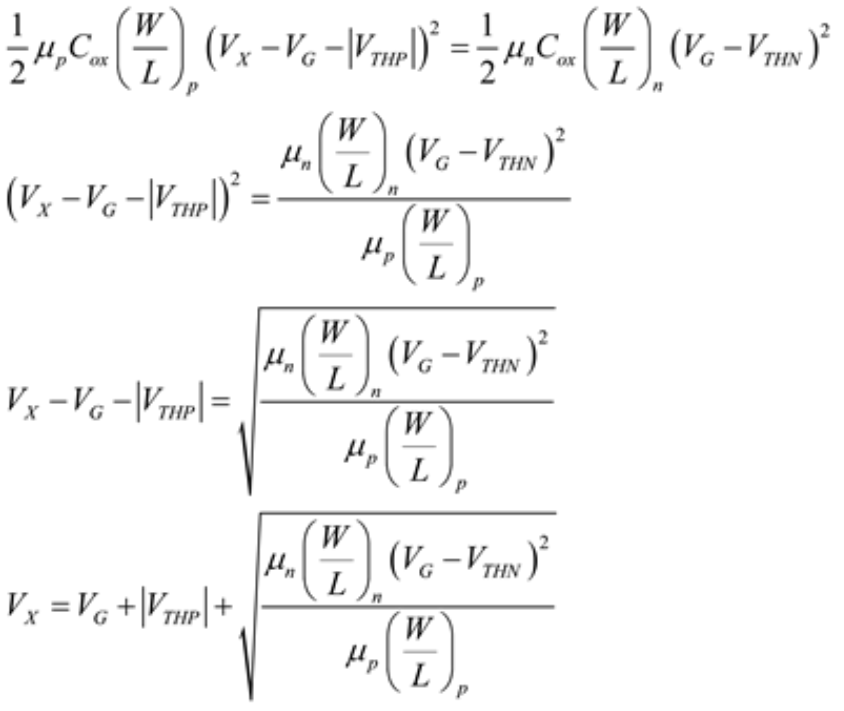
\includegraphics[width=1\linewidth]{2.24-10}
	\end{minipage}
\end{figure}

\begin{figure}[H] %H为当前位置,!htb为忽略美学标准,htbp为浮动图形
	\begin{minipage}{\linewidth}
		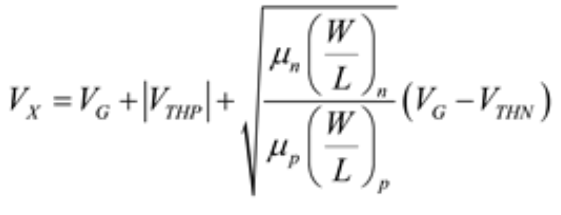
\includegraphics{2.24-11}
	\end{minipage}
\end{figure}

\begin{figure}[H] %H为当前位置,!htb为忽略美学标准,htbp为浮动图形
	\begin{minipage}{\linewidth}
		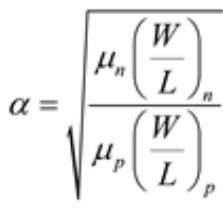
\includegraphics{2.24-12}
	\end{minipage}
\end{figure}

考虑$M_2$进线性区

$I_X=\frac{1}{2}\mu_nC_{ox}(\frac{W}{L})_n(V_G-V_{THN})^2$

对$V_G+|V_{THP}|<V_X<V_G+|V_{THP}|+\alpha(V_G-V_{THN})$:

$I_X=\frac{1}{2}\mu_pC_{ox}(\frac{W}{L})_p(V_{X}-V_G-|V_{THP}|)^2$

\begin{figure}[H] %H为当前位置,!htb为忽略美学标准,htbp为浮动图形
	\begin{minipage}{\linewidth}
		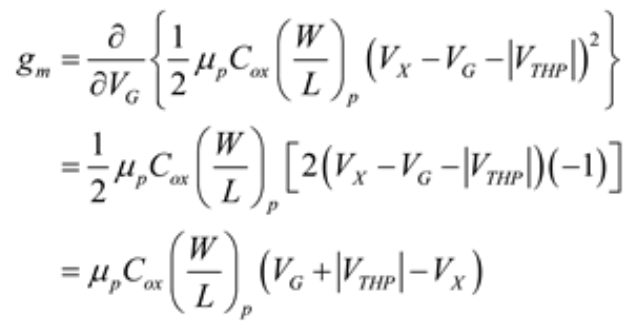
\includegraphics{2.24-13}
	\end{minipage}
\end{figure}

对$V_G+|V_{THP}|+\alpha(V_G-V_{THN})<V_X$:

$I_X=\frac{1}{2}\mu_nC_{ox}(\frac{W}{L})_n(V_G-V_{THN})^2$

\begin{figure}[H] %H为当前位置,!htb为忽略美学标准,htbp为浮动图形
	\begin{minipage}{\linewidth}
		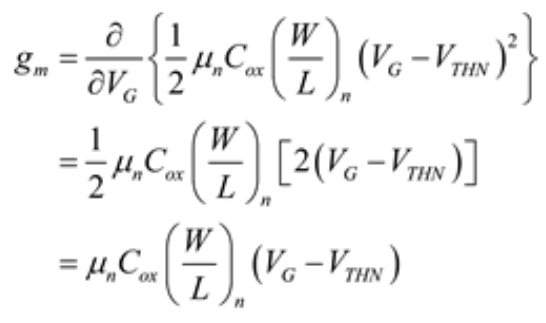
\includegraphics{2.24-14}
	\end{minipage}
\end{figure}

		\begin{figure}[H] %H为当前位置,!htb为忽略美学标准,htbp为浮动图形
	\begin{minipage}{\linewidth}
		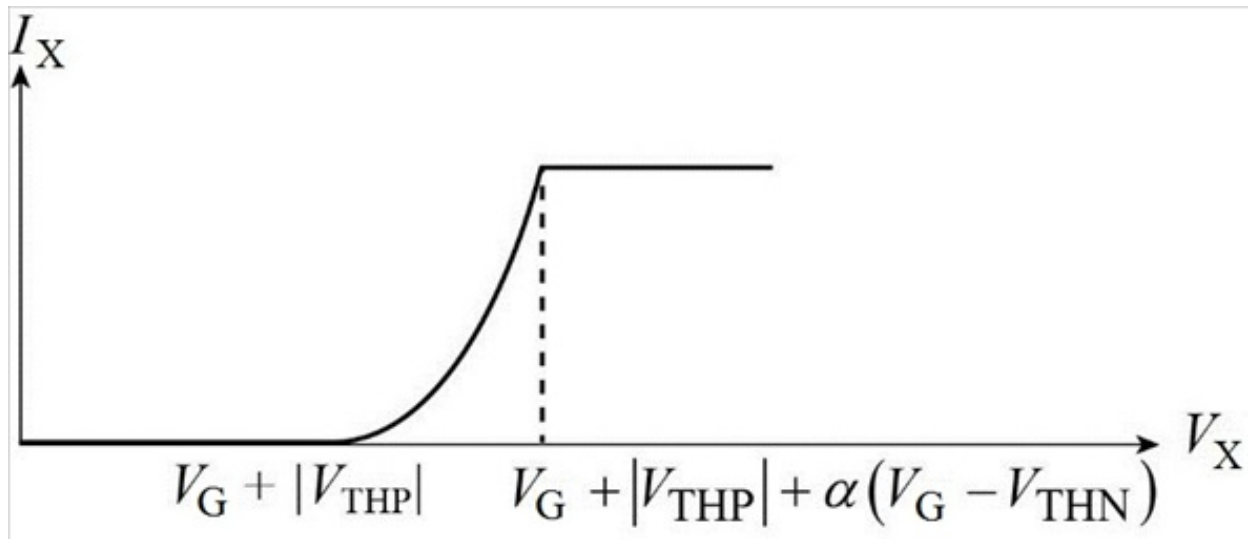
\includegraphics[width=1\linewidth]{2.24-15}
	\end{minipage}
	\caption*{图7} %最终文档中希望显示的图片标题
\end{figure}

\begin{figure}[H] %H为当前位置,!htb为忽略美学标准,htbp为浮动图形
	\begin{minipage}{\linewidth}
		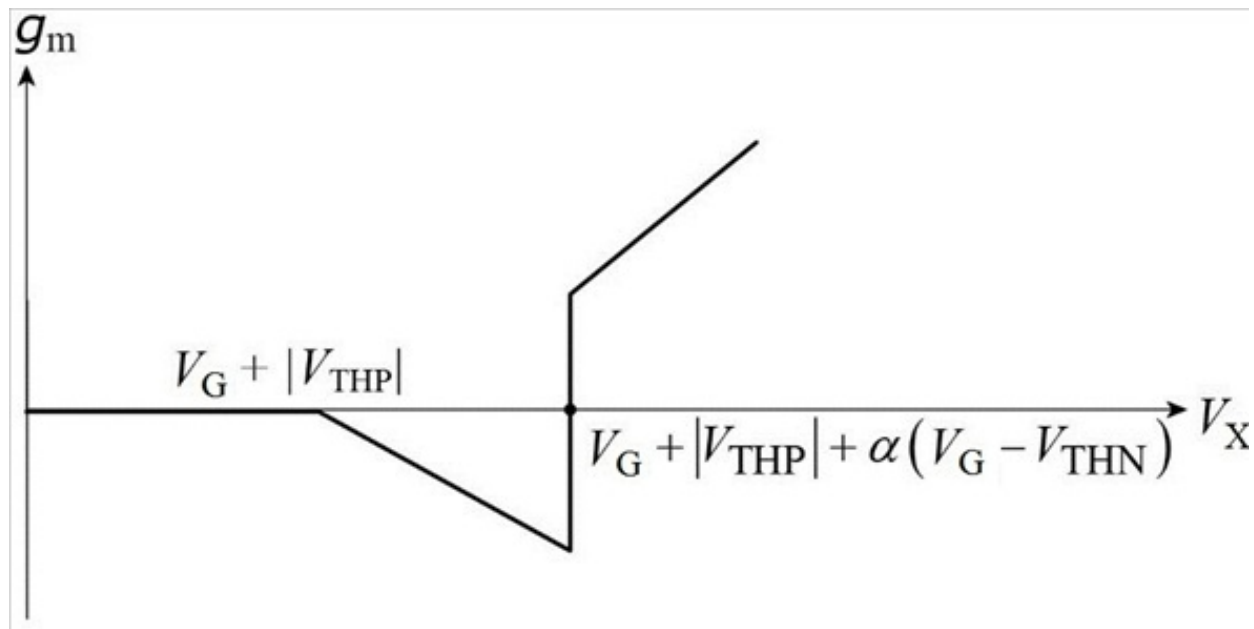
\includegraphics[width=1\linewidth]{2.24-16}
	\end{minipage}
	\caption*{图8} %最终文档中希望显示的图片标题
\end{figure}














